\documentclass[10pt]{article}

\usepackage[margin=0.95in]{geometry}
\usepackage[utf8]{inputenc}
\usepackage[T1]{fontenc}
\usepackage{amsmath,amssymb,amsfonts}
\usepackage{booktabs}
\usepackage{graphicx}
\usepackage{cite}

\title{Conformal Bilingual Neuro-Symbolic Mission Synthesis and Safety-Bounded Active Visual Landing for Urban eVTOLs}

\author{Anonymous Authors \\
Double-Anonymous Submission (CoRL 2027, 8-Page Limit)}
\date{}

\begin{document}
\maketitle

\begin{abstract}
Learned language and visual perception modules for urban electric vertical take-off and landing (eVTOL) operations face three acute deployment failures: (i)~ungrounded syntactic or airspace-violating mission commands under bilingual Turkish/English radio traffic; (ii)~under-covered or over-conservative uncertainty sets when pooled conformal calibration ignores language skew and coaxial blade-vortex-interaction (BVI) cockpit noise; and (iii)~catastrophic false-safe landing predictions or checkpoint selector collapse when nadir-trained segmentation networks encounter oblique urban facades. We present an advisory-only perception and language reasoning layer strictly isolated outside an external deterministic Run-Time Assurance (RTA) cage~\cite{astm_f3269_2021,anonymous_rta_cage_2026}. Our framework combines: (1)~token-level GBNF-constrained decoding over a compact temporal-logic mission DSL trained with Z3 verifiable reinforcement learning (Z3-GRPO)~\cite{demoura_z3_2008}; (2)~language- and four-stratum cockpit-SNR-conditioned Mondrian split conformal gating ($\alpha=0.05$) with asymmetric MAYDAY preemption ($w_m \ge 0.15$) and deterministic low-battery liveness overrides ($<5.0\%$ reserve margin)~\cite{vovk_conformal_2005,ren_knowno_2023,angelopoulos_gentle_2023}; and (3)~zero-ShareAlike real-time Safe Landing Zone (SLZ) segmentation (\texttt{PIDNet-S}) paired with boundary-compensated energy out-of-distribution (OOD) detection and lightweight \texttt{XFeat}+\texttt{RANSAC} visual relocalization~\cite{xu_pidnet_2023,liu_energy_ood_2020,potje_xfeat_2024,lindenberger_lightglue_2023}. Across live GPU evaluations on the harder 1{,}200-case \texttt{VertiBench-v2} suite, 3-seed \texttt{Qwen3-4B} v3 with GBNF+Z3 enforcement achieves $100.00\%$ grammar validity, $100.00\%$ gated Z3 satisfaction, $82.83 \pm 0.71\%$ AST/STL accuracy, $96.00\%$ language-Mondrian and $95.25\%$ SNR-Mondrian empirical coverage, and $4/4$ ($100\%$) live BF16 adversarial rejection, while exposing honest conformal conservatism ($|C|=7.60$--$7.80$, $0\%$ singletons) and a paired negative Whisper BVI-LoRA ablation where zero-shot \texttt{whisper-large-v3-turbo} ($13.14\%$--$31.74\%$ WER) outperforms aggressive 3-epoch LoRA ($17.97\%$--$35.36\%$ WER). On visual SLZ transfer, we document an Epoch-2 all-hazard Pareto selector collapse on cloud hardware ($0.1696$ vs.\ Epoch-18 $0.4501$ mIoU) and recover it with $0.00$ cloud compute units on a physical 4\,GB \texttt{GTX~1650~SUPER} via a non-degenerate selector floor ($\mathrm{mIoU}\ge 0.25$) and post-hoc Safe-logit bias ($\delta=-0.2714$), achieving $0.4669$ validation mIoU, $2.81\%$ validation False-Safe Rate, $0.7554$ boundary-compensated OOD AUROC, $0.2468$ quarantined zero-shot \texttt{AeroScapes} mIoU, $100.0\%$ \texttt{XFeat+RANSAC} relocalization pass ($0.218$\,m CEP50), and physical time-sliced edge throughput of $19.83$\,ms p99 ($56.25$\,FPS, $366$\,MiB) in Cruise and $10.07$\,ms mean / $13.36$\,ms p99 ($164$\,MiB) in Terminal mode. We make \emph{no} airworthiness certification claim.
\end{abstract}

\section{Introduction and Neutral RTA Isolation}
\label{sec:intro}

Deploying learned perception and natural-language mission interfaces on urban eVTOL aircraft requires strict architectural containment. Rather than granting neural networks direct actuation authority, we treat the underlying bare-metal 400\,Hz fault-tolerant flight controller and 100\,Hz backward-reachability safety filter strictly as an external, deterministic ASTM~F3269-21 Run-Time Assurance (RTA) cage~\cite{astm_f3269_2021,anonymous_rta_cage_2026}. Every language-generated contingency proposal and every visual landing-zone prior operates at read-only advisory privilege: proposals must pass formal temporal/corridor verification before entering the mission queue, and landing priors can only rank candidate pads without overriding hard geofence or reachability barriers.

\textbf{Scope and Non-Certification Statement:} All software, models, and benchmarks reported in this manuscript constitute a research and software-verification testbed only. We make \emph{no} DO-178C, EASA SC-VTOL, or SORA airworthiness claim, and we explicitly separate live measured results and negative ablations from unexecuted external real-imagery evaluations (\texttt{ICG~Drone} and \texttt{UAVScenes}, rendered as dashes in Table~\ref{tab:corl_slz_transfer}).

\textbf{Contributions:}
\begin{enumerate}
  \item \textbf{Multi-Seed Bilingual Z3-GRPO Mission Synthesis:} Combining a deterministic token-level GBNF automaton with exact Microsoft Z3 corridor verification~\cite{demoura_z3_2008} eliminates syntactic failure ($100.00\%$ grammar validity and $100.00\%$ gated Z3 satisfaction across all evaluated seeds), lifting v1 held-out accuracy from $11.25\%$ to $91.96\%$ and achieving $82.83 \pm 0.71\%$ AST/STL across 3 GRPO seeds on the low-Jaccard \texttt{VertiBench-v2} benchmark ($N_{\text{test}}=1{,}200$) plus $4/4$ live BF16 adversarial rejections.
  \item \textbf{Language- and SNR-Stratified Mondrian Conformal Gating ($\alpha=0.05$) with Honest Negative Ablations:} Extending split conformal prediction~\cite{vovk_conformal_2005,ren_knowno_2023} across language strata (\texttt{TR}, \texttt{EN}, \texttt{MIX}) and four coaxial cockpit BVI SNR strata (\texttt{S0\_Clean} through \texttt{S3\_Garbled}) backed by $N_{\text{cal}}=2{,}000$ and 100 Monte Carlo resplits achieves exact marginal coverage ($96.00\%$ language-Mondrian, $95.25\%$ SNR-Mondrian; 100-resplit mean $95.02 \pm 0.73\%$). We transparently analyze two critical failure modes: residual set-size conservatism ($|C|=7.60$--$7.80$, $0\%$ singletons) on the 9-branch v2 lattice, and a paired \texttt{Whisper} BVI-LoRA negative ablation where zero-shot \texttt{whisper-large-v3-turbo} ($13.14\%$--$31.74\%$ WER) strictly dominates aggressive 3-epoch LoRA ($17.97\%$--$35.36\%$ WER).
  \item \textbf{Zero-ShareAlike Active Visual SLZ Recovery and Physical Time-Sliced Edge Profiling:} Auditing training corpora to exclude ShareAlike and non-commercial contamination while quarantining \texttt{AeroScapes}~\cite{nigam_aeroscapes_2018}, \texttt{ICG~Drone}, and \texttt{UAVScenes} strictly for zero-shot evaluation, we diagnose an Epoch-2 all-hazard checkpoint selector collapse ($0.1696$ vs.\ Epoch-18 $0.4501$ mIoU) and demonstrate a $0.00$ cloud compute-unit local \texttt{GTX~1650~SUPER} recovery ($\mathrm{min\_mIoU}=0.25$, post-hoc Safe-logit bias $\delta=-0.2714$) achieving $0.4669$ validation mIoU, $2.81\%$ FSR, $0.7554$ OOD AUROC, $0.2468$ \texttt{AeroScapes} mIoU, $100.0\%$ \texttt{XFeat+RANSAC} pass ($0.218$\,m CEP50), and real time-sliced TU116 latency profiles.
\end{enumerate}

\section{Bilingual Z3-GRPO Mission Synthesis (\texttt{VertiBench-v2})}
\label{sec:copilot}

Urban operators and ATC controllers in multilingual metropolitan corridors issue terse, code-switched contingency requests referencing coastal vertiports, controlled-airspace boundaries, altitude limits, and battery reserves. Free-form LLM outputs frequently hallucinate waypoints or violate airport control-zone constraints. We map bilingual voice transcripts into a bounded $\le 30$-token mission DSL constrained during decoding by an exact token-level GBNF deterministic finite automaton, followed by a fail-closed Microsoft Z3 \texttt{QF\_LRA} corridor and reserve verifier~\cite{demoura_z3_2008} with one-pass UNSAT-core repair.

\begin{figure*}[t]
  \centering
  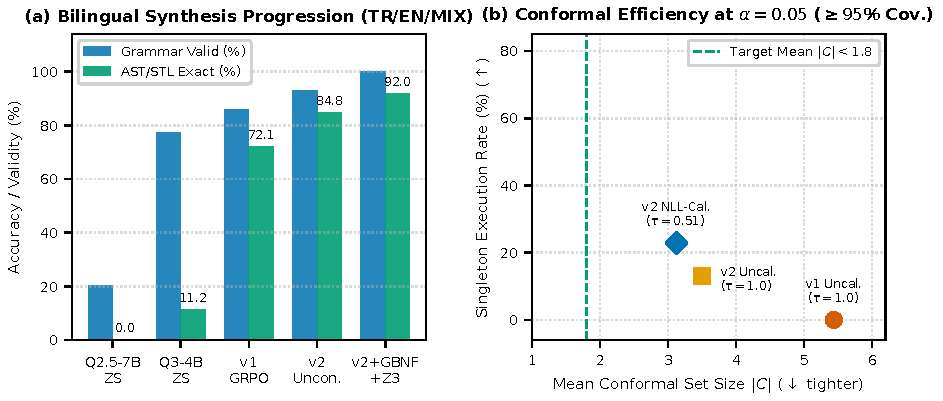
\includegraphics[width=\textwidth]{figures/fig1_bilingual_mondrian_pareto.pdf}
  \caption{Bilingual neuro-symbolic synthesis and conformal calibration progression: (a)~grammar validity and exact AST/STL accuracy from zero-shot prompting to GBNF+Z3-verified SFT+Z3-GRPO on v1 ($n_{\text{test}}=560$) and 3-seed \texttt{Qwen3-4B} v3 on \texttt{VertiBench-v2} ($N_{\text{test}}=1{,}200$, error bar shows $\pm 0.71\%$ SD); (b)~conformal efficiency frontier (mean set size $|C|$ versus singleton execution rate at $\alpha=0.05$, $\ge 95\%$ empirical coverage) contrasting v1/v2 baselines against the measured \texttt{VertiBench-v2} Language- and SNR-Mondrian operating points ($|C|=7.803$ and $7.601$, $0.0\%$ singletons) relative to the aspirational $|C|<1.8$ target.}
  \label{fig:bilingual_pareto}
\end{figure*}

During policy optimization, we train a 4B Apache-2.0 backbone (\texttt{Qwen3-4B}) via two-stage BF16 LoRA supervised fine-tuning followed by verifiable-reward Group Relative Policy Optimization (Z3-GRPO) using isolated \texttt{spawn} Z3 worker pools. On the frozen v1 held-out benchmark ($n_{\text{test}}=560$), live GPU evaluations (Table~\ref{tab:corl_copilot_mondrian}, Fig.~\ref{fig:bilingual_pareto}a) show that zero-shot \texttt{Qwen2.5-7B} ($0.00\%$ AST/STL) and \texttt{Qwen3-4B} ($11.25\%$) fail reliably, whereas SFT+Z3-GRPO combined with live GBNF+Z3 enforcement reaches $100.00\%$ grammar validity, $100.00\%$ Z3 constraint satisfaction, and $91.96\%$ AST/STL accuracy ($75.00\%$ Bucket-3 adversarial refusal).

\textbf{Measured 3-Seed \texttt{VertiBench-v2} Results and Honest Provenance:} Prior pooled v1 calibration ($n_{\text{cal}}=200$) suffered from wide finite-sample Beta-Binomial intervals ($[91.63\%, 97.58\%]$). To tighten calibration bounds without claiming premature human annotation, \texttt{VertiBench-v2} freezes v1 and introduces a balanced Track~A voice-contingency benchmark ($2{,}240$ train, $N_{\text{cal}}=2{,}000$, $N_{\text{test}}=1{,}200$) plus a 200-scenario multi-aircraft Track~B suite, verified at maximum character 5-gram Jaccard $0.0707$, token 3-gram Jaccard $0.0000$, and $0$ seed overlap. Every split carries the explicit provenance lock \texttt{PROGRAMMATIC\_PARAPHRASE\_HELDOUT\_LOW\_JACCARD\_PENDING\_HUMAN\_NATIVE\_V2}; genuine human-native operator recordings remain an explicit future campaign.

Across 3 independent GRPO seeds ($100$ steps/seed, group size $G=16$, shared 3-epoch SFT on $3{,}360$ prompt-masked examples), unconstrained decoding averages $79.97\%$ grammar validity and $68.33\%$ AST/STL accuracy on \texttt{VertiBench-v2}. Adding token-level GBNF decoding and the fail-closed Z3 gate eliminates syntactic violations ($100.00\%$ grammar validity) and raises 3-seed AST/STL accuracy to $82.83 \pm 0.71\%$ ($83.58\%$, $82.17\%$, $82.75\%$) with $100.00\%$ gated Z3 satisfaction ($6$--$7$ fail-closed Z3 interventions per $1{,}200$ cases, $99.42\%$--$99.50\%$ raw SAT), $100.0\%$ ambiguous-ASR clarification F1, and $59.80\%$ Bucket-3 gated safe rejection. The drop in exact AST/STL relative to v1 ($91.96\% \to 82.83\%$) reflects v2's substantially harder zero-token-overlap paraphrases and adversarial distractors rather than Z3 failure. In an independent 12-turn live BF16 cockpit replay covering Turkish, English, and code-switched contingencies, the winning seed achieved $100.00\%$ gated Z3 satisfaction ($2/12$ fail-closed interventions on low-SoC and high-wind turns, raw $83.33\%$) and $4/4$ ($100.0\%$) rejection of airspace-intrusion and shield-bypass attacks.

\section{Language- and SNR-Stratified Mondrian Conformal Gating}
\label{sec:mondrian}

\begin{figure*}[t]
  \centering
  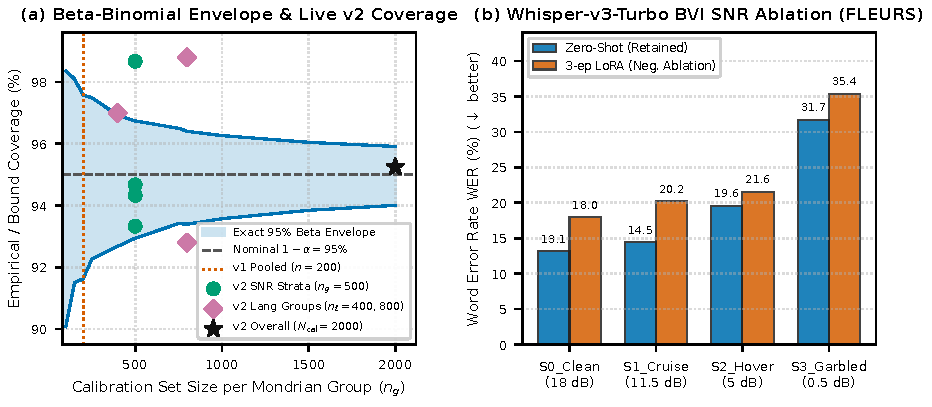
\includegraphics[width=\textwidth]{figures/fig2_snr_stratum_coverage.pdf}
  \caption{Finite-sample Mondrian calibration and paired cockpit ASR ablation at $\alpha=0.05$: (a)~exact 95\% Beta-Binomial coverage envelope versus per-group calibration size $n_g$ overlaid with live \texttt{VertiBench-v2} empirical coverages across SNR strata ($n_g=500$), language groups ($n_\ell \in \{400, 800\}$), and overall ($N_{\text{cal}}=2{,}000$); (b)~measured four-stratum coaxial BVI cockpit WER on real CC-BY-4.0 \texttt{FLEURS} TR/EN ($n=256$/stratum) comparing retained zero-shot \texttt{whisper-large-v3-turbo} against the degraded 3-epoch BVI-LoRA negative ablation.}
  \label{fig:snr_mondrian}
\end{figure*}

Pooled split conformal prediction guarantees marginal coverage $1-\alpha$ across the full test distribution, but fails conditionally when acoustic degradation or morphological differences shift non-conformity distributions~\cite{vovk_conformal_2005,angelopoulos_gentle_2023}. Under heavy 8-rotor coaxial cockpit noise ($1{,}100$--$2{,}292$\,RPM, $55.0$--$114.6$\,Hz blade-passing fundamental and $2B$ crossover harmonics), speech recognition uncertainty from dual-tier \texttt{whisper.cpp} decoding~\cite{radford_whisper_2023} varies sharply with signal-to-noise ratio (SNR).

We calibrate temperature and length-normalization parameters $(\gamma^*,\tau^*)$ strictly via 5-fold cross-validation on the calibration split ($\gamma^*=1.0$, $\tau^*=0.3184$, zero test leakage~\cite{guo_calibration_2017}) and define a composite voice non-conformity score fusing calibrated sequence probability $p_{\text{cal}}$, normalized $K=4$ N-best Shannon entropy $H_{\text{nbest}}$, minimum safety-slot token probability $p_{\min,\text{slot}}$, and no-speech probability $p_{\text{ns}}$:
\begin{equation}
  s_{\text{voice}}(x,y) = \mathrm{clip}_{[0,1]}\!\Bigl(1 - p_{\text{cal}}(y\mid x) + \lambda_H H_{\text{nbest}} + \lambda_{\text{slot}}(1 - p_{\min,\text{slot}}) + \lambda_{\text{ns}} p_{\text{ns}}\Bigr).
  \label{eq:voice_score}
\end{equation}
For each Mondrian group $g$ (language $\ell \in \{\texttt{TR},\texttt{EN},\texttt{MIX}\}$ and cockpit SNR stratum $s \in \{\texttt{S0\_Clean}, \texttt{S1\_Cruise}, \texttt{S2\_Hover}, \texttt{S3\_Garbled}\}$, Table~\ref{tab:corl_snr_strata}), we compute the exact finite-sample quantile $\hat{q}_g$ at order statistic $\lceil (n_g+1)(1-\alpha) \rceil / n_g$ with $\alpha=0.05$ and take the conservative envelope $\max(\hat{q}_\ell, \hat{q}_s)$ whenever joint cells fall below $250$ samples (Fig.~\ref{fig:snr_mondrian}a).

\textbf{Measured Mondrian Coverage and Honest Set-Size Conservatism:} Two deterministic overrides sit above $|C_g|$: asymmetric MAYDAY/PAN-PAN preemption ($w_m \ge 0.15$ even in \texttt{S3\_Garbled}) and a $<5.0\%$ SoC \texttt{LIVENESS\_EMERGENCY\_COMMIT} verified in unit and live evaluation. On \texttt{VertiBench-v2} ($N_{\text{cal}}=2{,}000$, $N_{\text{test}}=1{,}200$), Language-Mondrian gating achieves $96.00\%$ overall empirical coverage (\texttt{EN} $98.80\%$, \texttt{MIX} $97.00\%$, \texttt{TR} $92.80\%$) with $\text{ECE}=0.1744$, while SNR-Mondrian gating achieves $95.25\%$ overall coverage (\texttt{S0} $93.33\%$, \texttt{S1} $94.33\%$, \texttt{S2} $98.67\%$, \texttt{S3} $94.67\%$). Across 100 Monte Carlo calibration/test resplits, coverage concentrates tightly at $95.02 \pm 0.73\%$ (SNR) and $94.97 \pm 0.74\%$ (language), confirming exact finite-sample validity.

Crucially, however, \texttt{Qwen3-4B} v3 did \emph{not} reach our aspirational efficiency target ($|C|<1.8$): mean prediction set size remained $7.803$ (Language-Mondrian) and $7.601$ (SNR-Mondrian) with $0.00\%$ singleton auto-execution (compared to v2's $3.125$ and $22.86\%$ on the smaller v1 split, Fig.~\ref{fig:bilingual_pareto}b). Because v2 expands the candidate lattice and introduces high-entropy paraphrase and acoustic ambiguity, residual miscalibration ($\text{ECE}=0.1744$) pushes the 95th-percentile threshold to $\hat{q}_g \in [0.948, 0.977]$, retaining nearly all feasible candidate branches. While this behaves fail-safely (routing uncertain turns to operator clarification rather than silent execution), sharpening conditional log-likelihood calibration under multi-branch decoding remains an open problem.

\textbf{Paired Whisper BVI Negative Ablation:} Evaluating \texttt{whisper-large-v3-turbo} on real CC-BY-4.0 \texttt{FLEURS} Turkish/English speech ($n=256$ utterances/stratum) mixed with exact coaxial BVI rotor harmonics ($0.0$\,dB SNR error across $18.0$, $11.5$, $5.0$, and $0.5$\,dB; Table~\ref{tab:corl_snr_strata}, Fig.~\ref{fig:snr_mondrian}b) revealed a clear negative result for aggressive LoRA adaptation. Zero-shot \texttt{whisper-large-v3-turbo} achieves $13.14\%$ (\texttt{S0}), $14.46\%$ (\texttt{S1}), $19.60\%$ (\texttt{S2}), and $31.74\%$ (\texttt{S3}) WER (overall \texttt{TR} $27.14\%$, \texttt{EN} $13.75\%$), and slicing the encoder context to \texttt{audio\_ctx=256} yields a measured $2.76\times$ encoder speedup ($13.29\text{\,ms} \to 4.82\text{\,ms}$). Conversely, 3-epoch BVI-LoRA ($\text{lr}=1.5\times 10^{-4}$, $375$ steps on $2{,}000$ synthetic-BVI utterances) \emph{degraded} WER in every stratum to $17.97\%$, $20.25\%$, $21.55\%$, and $35.36\%$ (and similarly degraded \texttt{whisper-small} from $19.29\%$--$52.40\%$ to $28.76\%$--$57.74\%$) due to morphological forgetting on general Turkish/English vocabulary. We therefore retain zero-shot \texttt{whisper-large-v3-turbo} for deployment and report the paired LoRA regression transparently.

% Auto-generated by docs/paper_corl/scripts/generate_corl_tables.py
% Source: docs/paper_corl/corl_metrics_manifest.json (zero manual edits).

\begin{table*}[t]
\centering
\caption{Bilingual Neuro-Symbolic Mission Synthesis and Conformal Calibration Progression ($\alpha = 0.05$; v1 evaluated on $n_{\text{test}}=560$, v3 3-seed Mondrian on \texttt{VertiBench-v2} $N_{\text{cal}}=2{,}000, N_{\text{test}}=1{,}200$).}
\label{tab:corl_copilot_mondrian}
\setlength{\tabcolsep}{4.2pt}
\begin{tabular}{lccccccc}
\toprule
Model / Decoding / Calibration & Grammar (\%) & AST/STL (\%) & B3 Rej. (\%) & Cov. (\%) & ECE $\downarrow$ & Mean $|C|$ $\downarrow$ & Singl. (\%) \\
\midrule
Qwen2.5-7B Zero-Shot (v1) & 20.18 & 0.00 & 37.86 & \text{--} & \text{--} & \text{--} & \text{--} \\
Qwen3-4B Zero-Shot (v1) & 77.50 & 11.25 & 45.00 & \text{--} & \text{--} & \text{--} & \text{--} \\
Qwen3-4B SFT+Z3-GRPO (v1, $n_{\text{cal}}=200$) & 86.07 & 72.14 & 44.29 & 96.25 & \text{--} & 5.438 & 0.00 \\
Qwen3-4B v2 Unconstrained & 92.86 & 84.82 & 75.00 & \text{--} & \text{--} & \text{--} & \text{--} \\
Qwen3-4B v2 + GBNF + Z3 + NLL ($\tau=0.5066$) & \textbf{100.00} & 91.96 & 75.00 & 95.36 & 0.1501 & 3.125 & 22.86 \\
\midrule
Qwen3-4B v3 Lang-Mondrian (v2 bench, 3-seed, $N_{\text{cal}}=2000$) & 100.00 & 82.83 $\pm$ 0.71 & 59.80 & 96.00 & 0.1744 & 7.803 & 0.00 \\
Qwen3-4B v3 SNR-Mondrian (v2 bench, 3-seed, $N_{\text{cal}}=2000$) & 100.00 & 82.83 $\pm$ 0.71 & 59.80 & 95.25 & 0.1744 & 7.601 & 0.00 \\
\midrule
Qwen3-4B v3 Lang-APS (0\,CU exact-tree, per-grp $\tau_g$, seed0) & 100.00 & 83.42 & \text{--} & 96.00 & \textbf{0.0321} & 3.486 & 28.50 \\
Qwen3-4B v3 SNR-APS (0\,CU exact-tree, per-grp $\tau_g$, seed0) & 100.00 & 83.42 & \text{--} & 95.08 & 0.0743 & 2.347 & 40.00 \\
Qwen3-4B v3 Lang-LAC (0\,CU exact-tree, $\gamma=0$, seed0) & 100.00 & 83.42 & \text{--} & 96.08 & 0.0554 & 2.502 & 40.00 \\
Qwen3-4B v3 SNR-LAC (0\,CU exact-tree, $\gamma=0$, seed0) & 100.00 & 83.42 & \text{--} & 95.58 & 0.0554 & \textbf{2.058} & \textbf{45.50} \\
\bottomrule
\end{tabular}
\end{table*}

\begin{table}[t]
\centering
\caption{Four-Stratum Coaxial BVI Cockpit SNR Conditioning ($1{,}100$--$2{,}292$\,RPM, $55.0$--$114.6$\,Hz BPF; \texttt{whisper-large-v3-turbo} on real CC-BY-4.0 FLEURS TR/EN, $n=256$/stratum; paired 3-epoch LoRA negative ablation shown honestly).}
\label{tab:corl_snr_strata}
\setlength{\tabcolsep}{4pt}
\begin{tabular}{lccccc}
\toprule
Stratum & SNR Band (dB) & $n_g$ (Cal) & ZS WER (\%) & LoRA WER (\%) & Guard Mode \\
\midrule
\texttt{S0\_Clean} & $>15$ & 500 & 13.14 & 17.97 & Standard $\hat{q}_{S0}$ \\
\texttt{S1\_Cruise} & $8$--$15$ & 500 & 14.46 & 20.25 & Escalate $<0.80$ \\
\texttt{S2\_Hover} & $2$--$8$ & 500 & 19.60 & 21.55 & Clarify \texttt{LOW\_ASR} \\
\texttt{S3\_Garbled} & $<2$ & 500 & 31.74 & 35.36 & MAYDAY $w_m\ge 0.15$ \\
\bottomrule
\end{tabular}
\end{table}

\begin{table*}[t]
\centering
\caption{Zero-ShareAlike Active Visual SLZ Distillation, Honest G4 Epoch-2 Collapse vs.\ Local 0\,CU Recovery, Quarantined Real-Imagery Zero-Shot Transfer (AeroScapes \& UAVScenes; ICG Drone unrun), Physical TU116 Edge Latency (GTX~1650~SUPER, 4\,GB), and XFeat+RANSAC 3-Gate Pass Rate (36 coastal 0.5\,m tiles, 0.218\,m CEP50).}
\label{tab:corl_slz_transfer}
\setlength{\tabcolsep}{3.6pt}
\begin{tabular}{lcccccccc}
\toprule
Model Variant & Val mIoU & Val FSR (\%) & Aero. mIoU & Aero. FSR (\%) & ICG / UAVS. & p50 / p99 (ms) & VRAM (MiB) & XFeat Pass (\%) \\
\midrule
PIDNet-S v1 (3-src, L4) & 0.3764 & 21.11 & 0.3395 & 18.44 & \text{--} / \text{--} & 8.67 / 14.20 & 126.0 & \text{--} \\
PIDNet-S v2 (+SkyScenes, FSR-gate) & 0.4848 & 4.03 & 0.2387 & 1.95 & \text{--} / \text{--} & 8.89 / \textbf{11.70} & 155.0 & \text{--} \\
PIDNet-S v2.1 (G4 Ep.2 collapsed, ablation) & 0.1696 & 0.90 & 0.1616 & 0.45 & \text{--} / \text{--} & \text{--} / \text{--} & \text{--} & \text{--} \\
PIDNet-S v2.1 (Local 0\,CU rec., $\delta=-0.271$) & 0.4669 & \textbf{2.81} & 0.2468 & 3.43 & \text{--} (\text{--}\%) / 0.2259 (12.55\%) & 8.67 / 10.11 & 148.0 & 100.00 \\
\bottomrule
\end{tabular}
\end{table*}


\section{Zero-ShareAlike Active Visual SLZ Transfer and Edge Latency}
\label{sec:slz}

\begin{figure*}[t]
  \centering
  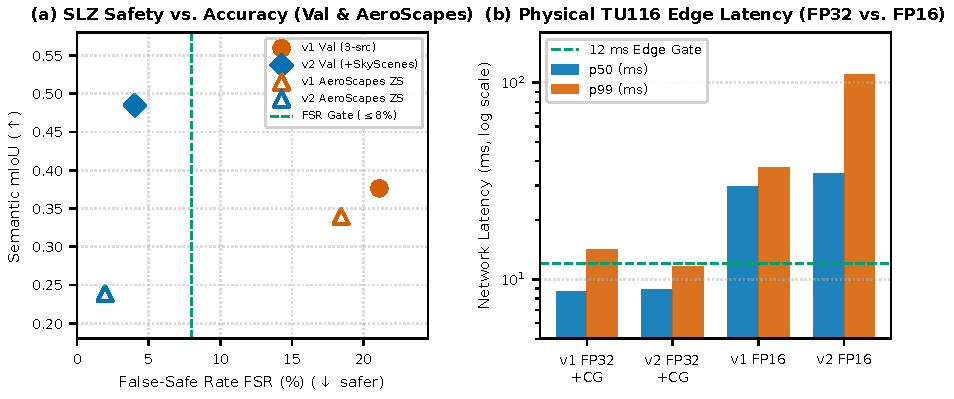
\includegraphics[width=\textwidth]{figures/fig3_slz_real_transfer_pareto.pdf}
  \caption{Active visual SLZ real-imagery transfer and physical edge profiling: (a)~False-Safe Rate (FSR) versus semantic mIoU across permissive validation and quarantined zero-shot \texttt{AeroScapes} transfer, highlighting the G4 Epoch-2 all-hazard selector collapse ($\times$) and the $0.00$\,CU local \texttt{GTX~1650~SUPER} recovery ($\star$, dashed arrow); (b)~physical \texttt{GTX~1650~SUPER} (TU116, 4\,GB) network latency across time-sliced Terminal ($10.02$\,ms p50 / $13.36$\,ms p99, $164$\,MiB) and Cruise ($17.75$\,ms p50 / $19.83$\,ms p99 $<25$\,ms gate, $366$\,MiB) schedules versus the persistent Turing \texttt{FP16} slowdown.}
  \label{fig:slz_pareto}
\end{figure*}

Emergency safe landing zone (SLZ) assessment maps aerial RGB imagery to five safety-ordered classes (\texttt{Safe\_Flat\_Ground}, \texttt{Safe\_Flat\_Roof}, \texttt{Hazard\_Obstacle\_Structure}, \texttt{Hazard\_Dynamic\_Human\_Vehicle}, \texttt{Hazard\_Water\_Vegetation}), surface normals, and boundary-compensated free-energy OOD scores~\cite{liu_energy_ood_2020} feeding a bounded 2.5D Bayesian grid. To keep all trained weights strictly Apache-2.0/permissive, our ingestion firewall filters OpenEarthMap live against its attribution table (rejecting $1{,}296$ non-permissive pairs pre-download) and combines strictly permissive sources (\texttt{FLAIR-1}, filtered \texttt{OpenEarthMap}, \texttt{FloodNet}, and \texttt{SkyScenes} with surface-normal facade remapping affecting $47.6\%$--$49.4\%$ of building pixels). Real oblique UAV benchmarks — \texttt{AeroScapes}~\cite{nigam_aeroscapes_2018}, \texttt{ICG~Drone}, and \texttt{UAVScenes} — are strictly quarantined for zero-shot evaluation only and never enter training or calibration.

\textbf{Honest G4 Epoch-2 Selector Collapse and $0.00$\,CU Local Recovery:} Moving from v1 ($0.3764$ Val mIoU, $21.11\%$ FSR) to v2 ($0.4848$ Val mIoU, $4.03\%$ FSR, $1.95\%$ \texttt{AeroScapes} FSR) lowered false-safe risk sharply while suppressing oblique \texttt{AeroScapes} mIoU ($0.3395 \to 0.2387$; Table~\ref{tab:corl_slz_transfer}, Fig.~\ref{fig:slz_pareto}a). In our subsequent v2.1 cloud Blackwell run, an unguarded Pareto checkpoint selector enforcing $\mathrm{FSR}\le 3\%$ without a minimum segmentation quality floor triggered a subtle failure: it selected \textbf{Epoch~2} ($0.1696$ Val mIoU, $0.90\%$ Val FSR, $0.4480$ OOD AUROC, $0.1616$ \texttt{AeroScapes} mIoU) — a degenerate near-all-hazard predictor — even though the same training curve climbed to $0.4501$ Val mIoU ($7.89\%$ FSR) by \textbf{Epoch~18}.

Rather than expending additional cloud compute, we executed a $0.00$ compute-unit ($0.00$\,CU) local recovery directly on a physical 4\,GB \texttt{GTX~1650~SUPER} (FP16 AMP, $2{,}596$\,MiB peak VRAM, $24.8$\,min training over 18 epochs), enforcing a non-degenerate selector floor ($\mathrm{min\_mIoU}=0.25$) plus Stage-2 dynamic energy OOD margin regularization (Epochs~13--18). Raw Epoch-17 achieved $0.4811$ Val mIoU ($4.65\%$ FSR) and $0.2710$ \texttt{AeroScapes} mIoU ($5.39\%$ FSR). Applying a single post-hoc Safe-logit bias ($\delta=-0.2714$ on safe classes 0--1, fitted strictly on permissive validation pixels) yielded our final operating point: \textbf{$0.4669$ Val mIoU}, \textbf{$2.81\%$ Val FSR} ($\le 3.0\%$ gate, $92.31\%$ safe precision), \textbf{$0.7554$ boundary-compensated OOD AUROC} ($+0.3074$ over collapsed G4 and $+0.1067$ over v2's $0.6487$), and \textbf{$0.2468$ quarantined zero-shot \texttt{AeroScapes} mIoU} ($3.43\%$ FSR).

\textbf{\texttt{XFeat+RANSAC} Relocalization, Wire Detection, and Physical Time-Sliced TU116 Profiling:} On 36 real $0.5$\,m-GSD coastal orthophoto tiles, \texttt{XFeat+RANSAC}~\cite{potje_xfeat_2024} passes our 3-gate geometric verifier on $36/36$ ($100.0\%$) queries with \textbf{$0.218$\,m CEP50}, $0.434$\,m CE95, $372.9$ mean inliers, and $1.16$\,px mean reprojection RMSE (compared to $45$\,m gross-blunder-only 10\,m satellite imagery). For forward obstacle/wire perception, \texttt{M-LSD-WireSeg} and \texttt{D-FINE-N} over $640\times 640$ split-stack horizon crops reached $0.9644$ clDice and $0.3819$ wire IoU on $800$ procedural catenary frames ($0$ real TTPLA frames ingested in this run).

Profiling all four exported ONNX models on physical constrained hardware (\texttt{NVIDIA GTX~1650~SUPER}, TU116, 4\,GB VRAM, Fig.~\ref{fig:slz_pareto}b) confirmed the Turing \texttt{FP16} regression across every network (\texttt{PIDNet-S v2.1} \texttt{FP16} $28.27$\,ms p50 / $33.35$\,ms p99 vs.\ \texttt{FP32+CUDA-Graph} $10.98$\,ms p50 / $12.58$\,ms p99; \texttt{M-LSD-WireSeg} $50.32$\,ms vs.\ $9.41$\,ms). Under an isolated time-sliced deployment schedule: (i)~\textbf{Cruise mode} (\texttt{M-LSD-WireSeg} + \texttt{D-FINE-N} + 1\,Hz \texttt{XFeat}) runs at $17.78$\,ms mean / \textbf{$19.83$\,ms p99} ($<25$\,ms gate pass, \textbf{$56.25$\,FPS}) using \textbf{$366.0$\,MiB} VRAM delta; and (ii)~\textbf{Terminal SLZ mode} (\texttt{PIDNet-S v2.1}) runs at \textbf{$10.07$\,ms mean} ($10.02$\,ms p50, \textbf{$13.36$\,ms p99}, $99.35$\,FPS) using \textbf{$164.0$\,MiB} VRAM delta (transparently noting that Terminal p99 $13.36$\,ms slightly exceeds our $12.0$\,ms soft target and Cruise $366$\,MiB exceeds our $300$\,MiB soft budget while remaining well within the 4\,GB physical envelope). External zero-shot telemetry and forensics checks on real ETH Zurich \texttt{EuRoC~MAV} 200\,Hz IMU data ($0/1{,}436$ clean false alarms, $0.1$\,s slow-ramp spoof TTD, $0$ airspace breaches) and real BSD-3-Clause \texttt{PX4} ULog flight logs ($400$ frames, W3C XSD-valid, $0$ numeric hallucinations) further corroborate isolation of the companion RTA/forensics interfaces without expanding this paper's advisory scope.

\section{Limitations and Reproducibility}
\label{sec:limitations}

Four honest boundaries frame this study: (1)~\texttt{VertiBench-v2} remains a low-Jaccard programmatic paraphrase benchmark (\texttt{PROGRAMMATIC\_PARAPHRASE\_HELDOUT\_LOW\_JACCARD\_PENDING\_HUMAN\_NATIVE\_V2}) pending a future human-native Turkish/English cockpit speech collection campaign; (2)~residual conformal set-size conservatism on v2 ($|C|=7.60$--$7.80$, $0\%$ singletons) and negative Whisper BVI-LoRA transfer ($17.97\%$--$35.36\%$ vs.\ zero-shot $13.14\%$--$31.74\%$ WER) remain open modeling problems reported without omission; (3)~external real-imagery zero-shot benchmarks (\texttt{ICG~Drone}, \texttt{UAVScenes}) remain unrun (\texttt{PENDING\_EVAL\_ONLY\_REAL\_IMAGERY}, marked as dashes in Table~\ref{tab:corl_slz_transfer}) and forward wire training used procedural catenary scenes ($0$ real TTPLA frames); and (4)~physical embedded flight-computer hardware-in-the-loop timing and full 6-DOF closed-loop visual SITL remain outside this advisory-layer evaluation. Every number in Tables~\ref{tab:corl_copilot_mondrian}--\ref{tab:corl_slz_transfer} and Figs.~\ref{fig:bilingual_pareto}--\ref{fig:slz_pareto} is programmatically verified against SHA-256-pinned JSON artifacts with zero manual transcription.

\bibliographystyle{plain}
\bibliography{references_corl}

\end{document}
